\anonsection{Задание 2}
\anonsubsection{Формулировка задания}
\begin{enumerate}
	\item Построить датчик сингулярного распределения, имеющий в качестве функции
     распределения канторову лесницу. С помощью критерия Колмогорова убедиться в
     корректности работы датчика.
	\item Для канторовых случайных величин проверить свойство симметричности
     относительно $ \frac{1}{2} $ ($ X $ и $ 1 - X $ распределены одинаково) и
     самоподобия относительно деления на 3 (условное распределение $Y$ при условии
     $ Y \in [0, 1/3] $ совпадает с распределением $ \frac{Y}{3} $) с помощью критерия
     Смирнова.
	\item Вычислить значение математическое ожидание и дисперсии для данного
     распределения. Сравнить теоритические значения с эмпирическими для разного объема
     выборок. Проиллюстрировать сходимость.
\end{enumerate}

\anonsubsection{Датчик канторова распределения}
Распределение, имеющее в качестве функции распределения канторову лестницу --- это
 распределение сосредоточенное на канторовом множестве или канторово распределение.
 Рассмотрим алгоритм построения канторова множества:\\
 Из единичного отрезка $ C_0=[0,1] $ удалим интервал $ (1/3,2/3) $.
 Оставшееся множество обозначим через $ C_1 $. Множество $ C_1=[0,1/3]\cup[2/3,1] $
 состоит из двух отрезков; удалим теперь из каждого отрезка его среднюю треть, и
 оставшееся множество обозначим через $ C_2 $. Повторив эту процедуру опять, удаляя
 средние трети у всех четырёх отрезков, получаем $ C_3 $. Действуя аналогично далее
 получаем последовательность вложенных множеств
 $ C_0 \supset C_1 \supset C_2 \supset C_3 \supset \dots $.

\begin{definition}
     Пересечение
	\[
	C = \bigcap\limits_{i = 0}^{\infty} C_i
	\]
	называется канторовым множеством.
\end{definition}

Из построения ясно, что канторово множество $ C $ можно определить как множество
 иррациональных чисел от нуля до единицы, представимое в троичной системе счисления
 лишь с помощью нулей и двоек. Это дает способ построения датчика канторова
 распределения.

\begin{equation}\label{cantor_detector}
     X = \displaystyle\sum_{i = 1}^{\infty} \dfrac{2}{3^i} \cdot Y_i, \quad i = 1,2,\dots,
\end{equation}

где $ Y_i \sim \mathrm{Bern(0.5)}. $\\
Для программной реализации датчика в таком случае можно использовать конечные суммы
 достаточно большого числа слагаемых. Сгенерируем $ n $ канторовых случайных
 величин и построим функцию распределения получившейся выборки (Рис. \eqref{fig:cantor_dist}). Отметим,
 что в силу возможности реализации лишь конечных сумм в \eqref{cantor_detector},
 среди параметров генератора присутствует eps, имеющий смысл минимальной
 ширины ступеньки в канторовой лестице.
 
 \begin{figure}[ht]
	\centering
	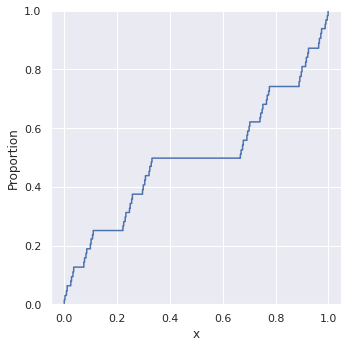
\includegraphics[width=0.7\linewidth]{"./resources/stairs.png"}
	\caption{Эмпирическая функция распределения сгенерированной выборки при $ n = 100 $}
     \label{fig:cantor_dist}
\end{figure}

\anonsubsection{Проверка корректности датчика и критерий Колмогорова}
Для проверки корректности построенного датчика воспользуемся
 критерием Колмогорова. Статистикой критерия является величина
\begin{equation}\label{kolm_statistic}
     D_n = \sup_{-\infty < x < \infty} | \hat{F}_n(x) - F(x)|,
\end{equation}
где $ \hat{F}_n(x) $ --- это выборочная функция распределения, а $ F(x) $
 --- функция распределения элементов выборки. Теорема Гливенко-Кантели
 утверждает, что для произвольной функции распределения $ F(x) $
 имеет место сходимость $ D_n \xrightarrow{\text{п.н.}} 0. $ Поэтому в случае,
 когда гипотеза соответствия верна, значение $ D_n $ для выборки достаточно
 большого размера слабо отклоняется от нуля.

Следующая теорема дает оценку для функции распределения величины
 $ \sqrt{n} D_n $ и позволяет таким образом оценивать вероятность
 наблюдаемого отклонения эмпирической функции распределения от теоретической.
\begin{theorem}[Теорема Колмогорова]
     Если функция распределения элементов выборки $ F(x) $ непрерывна, то
     для $ x > 0 $
     $$
     \displaystyle\lim_{n \to \infty}\mathbb{P}(\sqrt{n}D_n \le x) = K(x) = 1 +
     2 \displaystyle\sum_{k = 1}^{\infty}(-1)^k e^{-2k^2x^2}.
     $$
\end{theorem}
Таким образом проверка соответствия распределения может быть сведена
 к проверке $ K(\sqrt{n} D_n) $, где $ D_n $ формируется для конкретной
 выборки. При заданном уровне значимости $ \alpha $ гипотеза соответствия
 принимается при условии $ 1 - K(\sqrt{n} D_n) > \alpha. $

Так как функция распределения $ F(x) $ непрерывна и неубывает, а $ \hat{F}_n(x) $ ---
 кусочно-постоянна, то sup в \eqref{kolm_statistic} достигается в одной из точек
 разрыва функции $ \hat{F}_n $. Отсюда получаем формулу для вычисления
 $ D_n(x_1, \dots, x_n) $ заданной выборки $ (x_1, \dots, x_n) $:
$$
D_n(x_1, \dots, x_n) = \max_{1 \le i \le n} \left\{ \frac{i}{n} - 
 F(x_{(i)}), F(x_{(i)}) - \frac{i - 1}{n} \right\}.
$$
Здесь $ x_{(i)} $ --- $ i $-ый элемент выборки, сортированной по возрастанию. 

\anonsubsection{Свойство симметрии и самоподобия}
Покажем свойство симметрии канторова распределения. Пусть имеется канторова случайная
 величина $ X = \displaystyle\sum_{i = 1}^{\infty} \dfrac{2}{3^i} Y_i $, где $ Y_i
 \sim \mathrm{Bern}(0.5) $. Рассмотрим случайную величину $ 1 - X $:

$$ 
1 - X = 1 - \sum_{i = 1}^{\infty} \dfrac{2}{3^i} Y_i = \sum_{i = 1}^{\infty}
 \dfrac{2}{3^i} - \sum_{i = 1}^{\infty} \dfrac{2}{3^i} Y_i = \sum_{i = 1}^{\infty}
 \dfrac{2(1 - Y_i)}{3^i} = \sum_{i = 1}^{\infty} \dfrac{2}{3^i} Z_i. 
$$

Здесь $ Z_i \sim \mathrm{Bern}(0.5) $, поэтому случайные величины $ 1-X $ и $ X $
 распределены одинаково.

Покажем свойство самоподобия относительно деления на 3. Рассмотрим условное
 распредление канторовой случайной величины $ X $ на отрезке 
 $ \left[0; \dfrac{1}{3}\right] $. Это будет соответствовать тому, что
 $ Y_1 = 0 $. В таком случае:

$$ 
X = \sum_{i = 2}^{\infty} \dfrac{2}{3^i} Y_i = \sum_{i = 1}^{\infty}
 \dfrac{2}{3^{i+1}} Y_{i+1} = \left\{ Y_i = 0 \right\} = \dfrac{1}{3}
 \sum_{i = 1}^{\infty} \dfrac{2}{3^i} Y_i = \dfrac{1}{3} X.
$$

\anonsubsection{Проверка однородности и критерий Смирнова}
Пусть даны два набора наблюдений $ x_1, \dots, x_2 $ и $ y_1, \dots, y_m $,
 являющиеся реализациями некоторых наборов случайных величин $ X_1, \dots, X_n $
 и $ Y_1, \dots, Y_m $, относительно которых выполнены следующие утверждения:

\begin{enumerate}
     \item Случайные величины $ X_1, \dots, X_n $ независимы и имеют общую функцию
      распределения $ F(x) $.
     \item Случайные величины $ Y_1, \dots, Y_m $ независимы и имеют общую функцию
     распределения $ G(x) $.
     \item Обе функции $ F $ и $ G $ неизвестны, но являются непрерывными.
     \item Все компоненты случайного вектора $ (X_1, \dots, X_n, Y_1, \dots, Y_m) $
      независимы.
\end{enumerate}
\begin{definition}
     Два набора наблюдений, будем называть однородными, если для них выполнено:
     $$ G(x) = F(x) $$
     при всех $ x $.
\end{definition}

Для проверки гипотезы однородноси против альтернативы неоднородности
 в случае выполнения тверждениий (1)-(4) можно использовать критерий Смирнова,
 статистикой которого служит величина
$$
 D_{n, m} = \displaystyle\sup_x \left| \hat{F}_n(x) - \hat{G}_m(x) \right|,
$$
 где $ \hat{F}_n(x), \hat{G}_m(x) $ --- выборочные функции распределения,
 то есть $ D_{n,m} $ --- расстояние в равномерной метрике между эмпирическими
 функциями выборок.

Следующая теорема аналогично теореме Колмогорова дает оценку для функции
 распределения статистики $ \sqrt{\frac{nm}{n + m}} D_{n,m} $ и позволяет оценивать
 вероятность конкретного отклонения функций двух выборок.
\begin{theorem}[теорема Смирнова]
     Если гипотеза однородности верна, то при выполнении условий (1)-(4), для
      $ x > 0 $ имеет место:
	$$
		\lim\limits_{n, m \to \infty} \mathbb{P} \left( \sqrt{\dfrac{n m}{n + m}}
           D_{n,m} \le x \right) = K(x),
	$$
     где $ K(x) $ --- функция распределения Колмогорова из Теоремы 2.
\end{theorem}

Значения статистики на реализациях $ x_1, \dots, x_n $ и $ y_1, \dots, y_m $ можно
находить следующим способом:
$$
D_{n,m} = \max \left\{ D_{n,m}^+, D_{n,m}^- \right\},
$$
где
$$
D_{n,m}^+ = \sup_{x}(\hat{F}_n(x) - \hat{G}_m(x)) = \max_{1 \le i \le n}
\left\{ \frac{i}{n} - \hat{G}_m(x_{(i)}) \right\},
$$
$$
D_{n,m}^- = \sup_{x}(\hat{G}_m(x) - \hat{F}_n(x)) = \max_{1 \le j \le m}
\left\{ \frac{j}{m} - \hat{F}_n(y_{(j)}) \right\}.
$$

Применим критерий Смирнова для проверки свойства симметрии. Для
 этого сформируем две выборки из распределений $ X $ и $ 1 - X $ и применим для
 них критерий. Получим, что при n = 1000, eps = 0.00001 и уровне значимости
 $ \alpha = 0.05 $ гипотеза однородности принимается. Выборочные функции
 распределения $ X $ и $ 1 - X $ представлены на Рис. \eqref{subfig:symmetric}.
 Аналогично поступим для проверки свойства самоподобия. Выборочные функции
 соответствующих величин представлены на Рис. \eqref{subfig:self-similarity}.

 \begin{figure}
     \centering
     \begin{subfigure}[b]{0.45\textwidth}
         \centering
         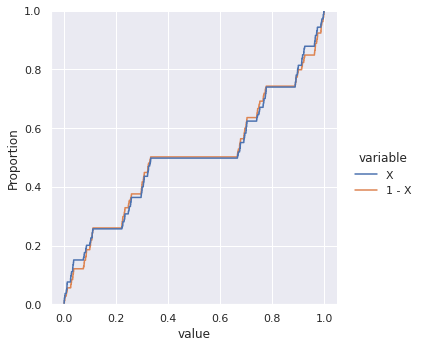
\includegraphics[width=\textwidth]{./resources/uniformity_1.png}
         \caption{Эмпирические функции распределения выбокок из $ X $ и $ 1 - X $}
         \label{subfig:symmetric}
     \end{subfigure}
     \hfill
     \begin{subfigure}[b]{0.45\textwidth}
         \centering
         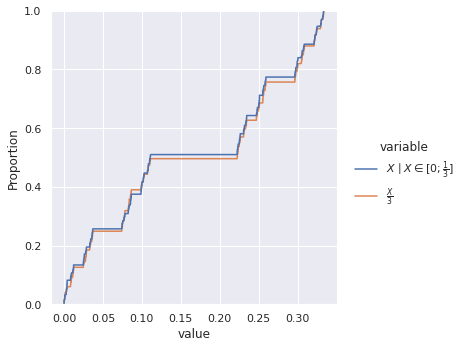
\includegraphics[width=\textwidth]{./resources/uniformity_2.png}
         \caption{Эмпирические функции распределения выбокок из
           $ X | X \in [0;\frac{1}{3}] $ и $ \frac{X}{3} $}
         \label{subfig:self-similarity}
     \end{subfigure}
     \caption{}
     \label{fig:cantor_properties}
\end{figure}

\anonsubsection{Математическое ожидание и дисперсия}
Вычислим математическое ожидание и дисперсию рассматриваемой случайной величины. 
Как упоминалось ранее, $ F $ обладает свойством самоподобия, то есть при
 $  0 < x < \dfrac{1}{3} $ выполнено соотношение $ F(x) = \dfrac{F(3x)}{2} $,
 а при $ \dfrac{2}{3} < x < 1 $ имеет место равенство $ F(x) = \dfrac{1}{2} +
 \dfrac{F(3x - 2)}{2} $. Поэтому

\begin{multline*}
\mathbb{E}[\xi] = \int\limits_{-\infty}^{+\infty} x \ dF(x) =
 \int\limits_{0}^{\frac{1}{3}} x \ dF(x) + \int\limits_{\frac{2}{3}}^{1} x \ dF(x) = \\
 \dfrac{1}{2} \int\limits_{0}^{\frac{1}{3}} x \ dF(3 x) + \dfrac{1}{2}
 \int\limits_{\frac{2}{3}}^{1} x \ d(\frac{1}{2} + F(3x - 2)).
\end{multline*}
Далее введем замену $y=3x$ в первом интеграле и $y=3x-2$ во втором интеграле:

\begin{multline*}
     \mathbb{E}[\xi] = \dfrac{1}{2} \int\limits_{0}^{1} \dfrac{y}{3} \ dF(y)
     + \dfrac{1}{2} \int\limits_{0}^{1} \dfrac{y+2}{3} \ dF(y) = \\
     = \dfrac{1}{6} \int\limits_{0}^{1} y \ dF(y) + \dfrac{1}{6}
     \int\limits_{0}^{1} y \ dF(y) + \dfrac{1}{3} \int\limits_{0}^{1} dF(y) =
     \dfrac{1}{3} \mathbb{E}[\xi] + \dfrac{1}{3}.
\end{multline*}
Таким образом, получаем $ \mathbb{E}[\xi] = \dfrac{1}{2} $.

Аналогичным способом с использованием свойства самоподобия вычислим дисперсию
 величины $ \xi $, используя вычисленное значения математического ожидания.
\begin{multline*}
     \mathbb{E}[\xi^2] = \int\limits_{0}^{\frac{1}{3}} x^2 \ dF(x) +
      \int\limits_{\frac{2}{3}}^{1} x^2 \ dF(x) = \dfrac{1}{2}\int\limits_{0}^{1}
      \left( \dfrac{y}{3} \right)^2 \ dF(y) + \dfrac{1}{2} \int\limits_{0}^{1}
      \left(\dfrac{y+2}{3}\right)^2dF(y) =\\
      = \dfrac{1}{9} \mathbb{E}[\xi^2] + \dfrac{2}{9} \mathbb{E}[\xi] + \dfrac{2}{9} =
      \dfrac{1}{9} \mathbb{E}[\xi^2] + \dfrac{1}{9} + \dfrac{2}{9}.
\end{multline*}
То есть имеем $ \mathbb{E}[\xi^2] = \dfrac{3}{8} $. Таким образом, получаем значение
 дисперсии $ \mathbb{D}[\xi] = \dfrac{3}{8} - \left( \dfrac{1}{2} \right)^2 =
  \dfrac{1}{8} $.

На Рис. \eqref{fig:convergence} демонстрируется сходимость выборочного матожидания
 и выборочной дисперсии к их теоретическим значениям, вычисленным выше, при увеличении
 размера выборки.

\begin{figure}[ht]
	\centering
	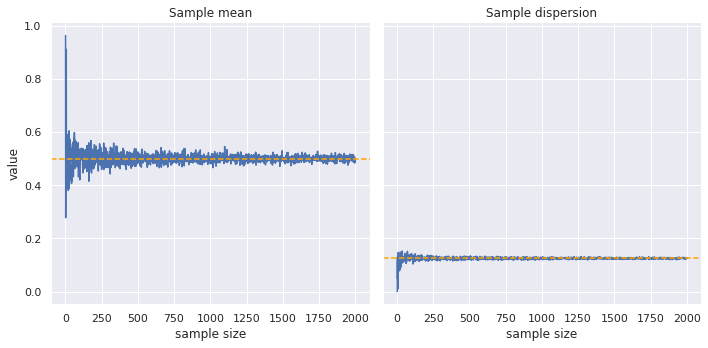
\includegraphics[width = 0.95\linewidth]{"./resources/convergence.png"}
	\caption{Сходимость выборочных значений матожидания и дисперсии к теоретическим.}
     \label{fig:convergence}
\end{figure}
